\section{Objetivos}
\begin{itemize}
    \item Medir los ángulos de incidencia, reflexión y refracción de un rayo de luz utilizando un disco óptico.
    \item Determinar experimentalmente el índice de refracción de diferentes medios utilizando el concepto de ángulo crítico y la aplicación de la Ley de Snell.
\end{itemize}

\section{Marco Teórico}
Cuando un rayo de luz incide sobre una interfase que separa dos medios con diferentes índices de refracción, parte de la luz se refleja y otra parte se refracta en el segundo medio. Esta interacción se describe a través de las leyes de reflexión y refracción.

\subsection{Leyes de Reflexión y Refracción}
La Ley de Reflexión establece que el ángulo de incidencia es igual al ángulo de reflexión, ambos medidos respecto a la normal a la interfase. Matemáticamente, se expresa como:
\[
\theta_i = \theta_r
\]
donde $\theta_i$ es el ángulo de incidencia y $\theta_r$ es el ángulo de reflexión.

La Ley de Snell describe la refracción de la luz al pasar de un medio a otro y se formula como:
\[
n_1 \sin(\theta_i) = n_2 \sin(\theta_t)
\]
donde $n_1$ y $n_2$ son los índices de refracción de los medios 1 y 2, respectivamente, y $\theta_t$ es el ángulo de transmisión.

\subsection{Reflexión Total Interna y Ángulo Crítico}
Cuando la luz pasa de un medio con un índice de refracción más alto a uno más bajo, existe un ángulo crítico de incidencia más allá del cual toda la luz se refleja internamente, sin refractarse al segundo medio. Este fenómeno se conoce como reflexión total interna. El ángulo crítico $\theta_c$ se puede calcular usando la relación:
\[
\theta_c = \arcsin\left(\frac{n_2}{n_1}\right)
\]
Esta situación ocurre solo cuando $n_1 > n_2$, lo que significa que la luz no puede pasar al medio con un índice de refracción menor si el ángulo de incidencia supera el ángulo crítico.

Estos principios fundamentales permiten entender cómo la luz interactúa con las superficies y se utiliza en una variedad de aplicaciones, desde la fibra óptica hasta la formación de imágenes ópticas.

\section{Análisis y discusión: Alineación del sistema}

\subsection{Verificar alineación}
\textbf{¿Cómo podría verificar en la práctica la debida alineación de este montaje? Piense en dos formas posibles.}
\begin{itemize}
  \item Realizar una comprobación visual del rayo láser asegurándose de que esté centrado y pase uniformemente a través del centro del disco óptico a lo largo de su trayecto.
  \item Utilizar un nivel de burbuja para asegurar que tanto el láser como el disco óptico estén nivelados horizontalmente, garantizando que el rayo láser incida perpendicularmente sobre el disco.
\end{itemize}

\subsection{¿Cómo no alterar?}
\textbf{¿Qué elementos del equipo podría mover y de qué modo, sin alterar la alineación del montaje?}
\begin{itemize}
    \item Ajustar la altura o la posición lateral del láser, siempre que el rayo siga incidiendo en el centro del disco óptico.
    \item Modificar la posición de la pantalla traslucida utilizada para visualizar el rayo láser, siempre que no se interrumpa el trayecto del rayo.
\end{itemize}

\subsection{Posición horizontal del disco}
\textbf{¿Es necesario que el disco óptico se encuentre en posición horizontal? Explique.}

Tener el disco óptico de este modo permite:
\begin{itemize}
    \item Facilita la medición precisa de los ángulos de incidencia y refracción, ya que la base de medición (el disco) está alineada con la gravedad, lo que ayuda a mantener la integridad de la perpendicularidad y los ángulos medidos.
    \item Previene distorsiones en las trayectorias del rayo causadas por una superficie inclinada, lo que podría afectar los resultados experimentales.
\end{itemize}

\section{Análisis y discusión: Ley de Snell - Interfase acrílico-aire}
\subsection{Montaje}
\textbf{Monte el semicilindro de acrílico y haga incidir un rayo sobre la superficie plana AB,
como lo muestra la Figura 4a. Note que A y B equidistan del centro del disco óptico.}

\subsection{¿Por qué no hay un desvío?}
\textbf{Si todo está bien, el rayo transmitido por la interfase plana AB no será desviado al
cruzar la interfase cilíndrica. ¿Por qué?}

La ausencia de desviación del rayo transmitido a través de la interfase plana AB al cruzar la interfase cilíndrica se debe a la orientación perpendicular del rayo respecto a esta superficie. Cuando el rayo de luz incide normalmente (perpendicularmente) sobre la interfase, no experimenta un cambio de dirección al pasar al otro medio, incluso si los índices de refracción son diferentes. Según la Ley de Snell, el ángulo de refracción depende directamente del ángulo de incidencia y de la relación entre los índices de refracción de los medios involucrados. Dado que el ángulo de incidencia es cero (incidencia normal), el rayo no se desvía, manteniendo su trayectoria a pesar de la transición entre medios con distintos índices de refracción.

\subsection{Tabla de Valores del semicilindro de acrílico aire}
\textbf{Mida el ángulo de incidencia $\theta_{i}$ y de transmisión $\theta_{t}$ correspondientes a la cara
plana AB. Anote los valores en la siguiente Tabla}

\begin{figure}[H]
  \centering
  \begin{subfigure}[b]{\textwidth}
      \centering
      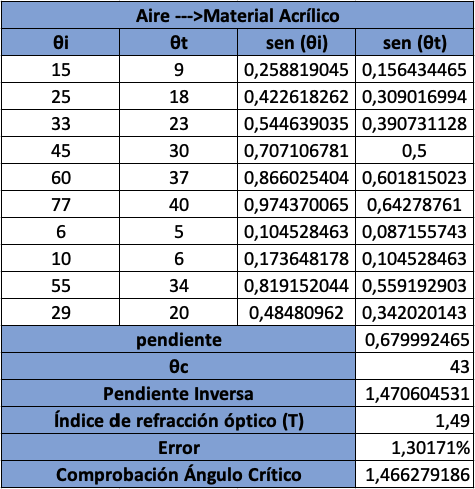
\includegraphics[width=0.55\textwidth]{Figures/1. Content/tabla1.png}
      \caption{Tabla de Valores del semicilindro de acrílico aire}
      \label{fig: Tabla 1}
  \end{subfigure}
  \hfill
\end{figure}


\subsection{$\theta_{i}$ vs $\theta_{t}$}
\textbf{Grafique $\theta_{i}$ vs $\theta_{t}$}

\begin{figure}[H]
  \centering
  \begin{subfigure}[b]{\textwidth}
      \centering
      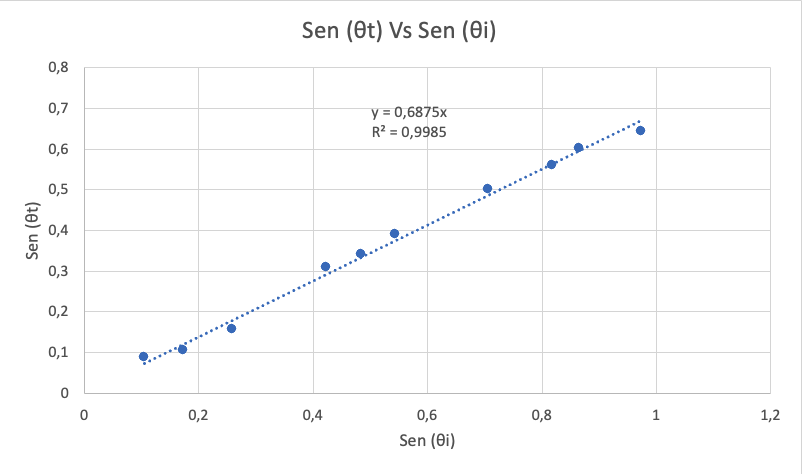
\includegraphics[width=0.7\textwidth]{Figures/1. Content/grafica1.png}
      \caption{$\theta_{i}$ vs $\theta_{t}$ de acrílico aire}
      \label{fig: Grafica 1}
  \end{subfigure}
  \hfill
\end{figure}

\subsection{Compare con la ecuación 2}
\textbf{¿Los valores del intercepto y la pendiente de la línea recta le parecen a simple vista
correctos? ¿Corresponden aproximadamente a los valores que debería obtener
según la ecuación (2)? Explique.}

La ecuación (2) a la que hacemos referencia es la Ley de Snell, que en forma matemática se expresa como:
\[
n_1 \sin(\theta_i) = n_2 \sin(\theta_t)
\]
donde \(n_1\) y \(n_2\) son los índices de refracción de los medios 1 y 2, respectivamente, y \(\theta_i\) y \(\theta_t\) son los ángulos de incidencia y de refracción.

En nuestro experimento, asumimos que el medio 1 es aire con \(n_1 \approx 1\), por lo que la ecuación se simplifica a:
\[
\sin(\theta_i) = n_2 \sin(\theta_t)
\]
Implicando que la pendiente de la gráfica de \(\sin(\theta_i)\) versus \(\sin(\theta_t)\) debería ser igual al índice de refracción del segundo medio, \(n_2\).

Aunque los valores experimentales obtenidos no coinciden perfectamente con los teóricos, se aproximan de manera razonable, destacando la influencia de factores experimentales en la precisión de los resultados obtenidos. Estas observaciones son esenciales para la comprensión práctica de la ley de Snell y subrayan la importancia de la precisión experimental en estudios de óptica física.

\subsection{Determinar el índice de refracción $n_{exp}$}
\textbf{Con base en el valor de este ángulo y la expresión (3), determine el índice de
refracción $n_{exp}$ del acrílico.}

Utilizando la pendiente inversa obtenida de la gráfica $\sin(\theta_i)$ vs $\sin(\theta_t)$, determinamos el índice de refracción experimental $n_{exp}$ del acrílico. La pendiente inversa, que es $1.47$, representa el índice de refracción del acrílico respecto al aire, dado que la relación $\frac{\sin(\theta_t)}{\sin(\theta_i)} = \frac{1}{n_{exp}}$.

\subsection{Comparar el índice de refracción $n_{exp}$ con $n_{teo}$}
\textbf{Compare el valor  $n_{exp}$ de este índice con el $n_{teo}$ que obtuvo anteriormente
mediante la gráfica \(\sin(\theta_i)\) vs \(\sin(\theta_t)\).}

Comparando el índice de refracción experimental $n_{exp} = 1.47$ con el índice teórico $n_{teo} = 1.49$, obtenido mediante la regresión lineal, observamos que estos valores son bastante cercanos, con un error porcentual de aproximadamente $1.30\%$. Esto indica una buena precisión experimental, aunque las pequeñas diferencias pueden ser atribuidas a factores como la precisión en la medición de los ángulos, calidad del equipo, o variaciones en las propiedades del material.

\subsection{Equidistar centro óptico}
\textbf{¿Considera fundamental que las aristas A y B del semicilindro equidisten del
centro del disco óptico? Explique.}

Es fundamental que las aristas A y B del semicilindro equidisten del centro del disco óptico para garantizar que el rayo de luz pase perpendicularmente a través del eje del semicilindro, lo cual es crucial para evitar desviaciones no deseadas del rayo debido a la refracción en ángulos no deseados. Esto asegura que las mediciones de los ángulos de incidencia y refracción se realicen bajo condiciones consistentes y controladas, contribuyendo así a la precisión del experimento.


\section{Análisis y discusión: Ley de Snell - Interfase agua-aire}
\subsection{Montaje}
\textbf{Reemplace el semicilindro de acrílico por el semicilindro hueco lleno de agua, y
repita los pasos anteriores para determinar ahora el índice de refracción del agua.}

\subsection{Tabla de Valores del semicilindro de agua-aire}
\textbf{Mida el ángulo de incidencia $\theta_{i}$ y de transmisión $\theta_{t}$ correspondientes de la siguiente Tabla}

\begin{figure}[H]
  \centering
  \begin{subfigure}[b]{\textwidth}
      \centering
      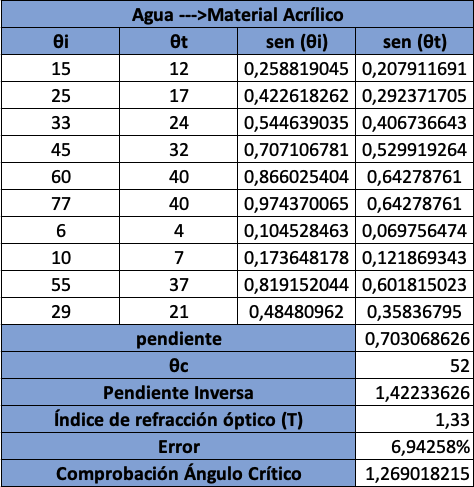
\includegraphics[width=0.55\textwidth]{Figures/1. Content/tabla2.png}
      \caption{Tabla de Valores del semicilindro de agua-aire}
      \label{fig: Tabla 2}
  \end{subfigure}
  \hfill
\end{figure}


\subsection{$\theta_{i}$ vs $\theta_{t}$}
\textbf{Grafique $\theta_{i}$ vs $\theta_{t}$}

\begin{figure}[H]
  \centering
  \begin{subfigure}[b]{\textwidth}
      \centering
      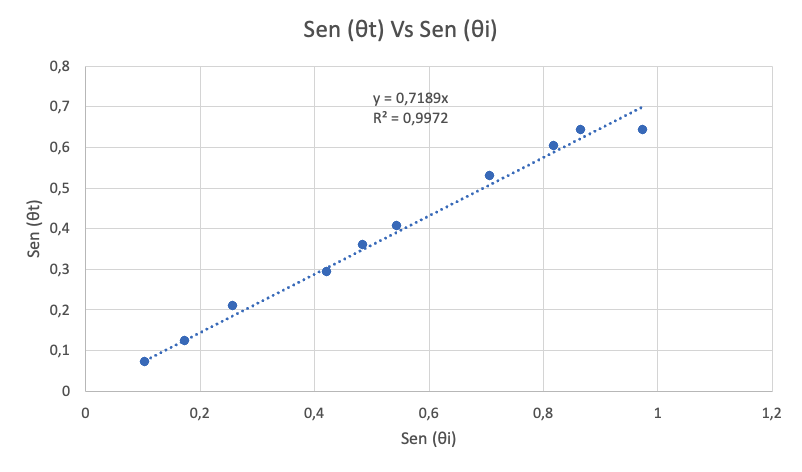
\includegraphics[width=0.7\textwidth]{Figures/1. Content/grafica2.png}
      \caption{$\theta_{i}$ vs $\theta_{t}$ de agua-aire}
      \label{fig: Grafica 2}
  \end{subfigure}
  \hfill
\end{figure}

\subsection{Determinar el índice de refracción $n_{exp}$}
\textbf{Con base en el valor de este ángulo y la expresión (3), determine el índice de
refracción $n_{exp}$ del acrílico.}

El índice de refracción experimental $n_{exp}$ del acrílico, utilizando la interfaz agua-aire, se determina por la pendiente inversa obtenida de la gráfica de $\sin(\theta_i)$ contra $\sin(\theta_t)$, que es aproximadamente $1.423$. Esto sugiere que el índice de refracción del medio entre el agua y el aire, considerando la presencia del acrílico, es de $1.423$.

\subsection{Calcular error}
\textbf{Calcule el porcentaje de error asociado con esta medición, tomando $1.33$ como el
valor teórico del índice de refracción del agua.}

El valor teórico del índice de refracción del agua es generalmente aceptado como $1.33$. El error porcentual entre el índice experimental y el teórico se calcula de la siguiente manera:
\[
\text{Error \%} = \left| \frac{n_{exp} - n_{teo}}{n_{teo}} \right| \times 100 = \left| \frac{1.422 - 1.33}{1.33} \right| \times 100 \approx 6.94\%
\]
Este cálculo muestra que hay un error aproximado del $6.94\%$ en la medición del índice de refracción experimental comparado con el valor teórico del agua.

\subsection{Pared gruesa de acrílico}
\textbf{Observe que entre el agua y el aire hubo una pared gruesa de acrílico, con un índice
de refracción distinto al del agua. ¿Por qué no se tuvo en cuenta este hecho al
determinar el ángulo crítico de la interfase agua-aire?}

A pesar de la presencia de una pared gruesa de acrílico entre el agua y el aire, el ángulo crítico y las mediciones de refracción se realizaron asumiendo que sólo se trataba de la interfaz agua-aire. Esto es común en experimentos educativos debido a la simplicidad y las limitaciones del equipo de medición. En un contexto más preciso o en investigaciones avanzadas, el efecto del acrílico se debería considerar, ya que altera la trayectoria y la refracción de la luz al pasar de un medio a otro, afectando el resultado final del índice de refracción observado.

\section{Causas de Error}
Las causas de error en este experimento sobre la ley de Snell podrían incluir:
\begin{itemize}
    \item La precisión en la medición de los ángulos, que depende fuertemente de la alineación del disco óptico y la calidad del equipo de medición.
    \item Variaciones en la calidad óptica del acrílico y el agua, que pueden alterar los índices de refracción y afectar las mediciones del ángulo crítico.
    \item Presencia de burbujas de aire o impurezas en los medios acrílico y agua, que pueden causar dispersión o desviación no uniforme de la luz.
    \item Influencia de la luz ambiental y reflexiones adicionales dentro del laboratorio que podrían interferir con la trayectoria del rayo de luz.
    \item La estimación errónea del ángulo crítico debido a una interpretación visual inexacta del fenómeno de la reflexión total interna.
\end{itemize}

\section{Conclusiones}
Basado en los experimentos realizados, se concluye que:
\begin{itemize}
    \item Los resultados obtenidos confirmaron las predicciones de la Ley de Snell sobre la relación entre los ángulos de incidencia y refracción y los índices de refracción de los medios involucrados.
    \item El uso de la ley de Snell permitió determinar con éxito los índices de refracción experimentales de acrílico y agua, demostrando la utilidad de esta ley en aplicaciones prácticas de óptica.
    \item Se observó una buena correlación entre los índices de refracción teóricos y experimentales, aunque con ligeras desviaciones que pueden ser atribuidas a las causas de error identificadas.
    \item Este experimento subraya la importancia de la precisión en la configuración experimental y la medición en estudios de óptica para obtener resultados fiables.
    \item Finalmente, el experimento proporcionó una experiencia práctica valiosa en la manipulación y medición de fenómenos ópticos, reforzando la comprensión teórica de la reflexión y la refracción de la luz en diferentes interfaces.
\end{itemize}
